% A1 research poster. Compile with pdfLaTeX (the Overleaf default).
%
% Every piece of text is 25 pt or larger: all LaTeX size commands are
% redefined below, so nothing can drop under the 24 pt minimum by accident.
% Figures are vector PDFs made at their printed width by
% scripts/06_poster_figures.py, so their 24 pt labels print at 24 pt.
\documentclass{article}

\usepackage[paperwidth=594mm, paperheight=841mm,
            left=20mm, right=20mm, top=16mm, bottom=14mm]{geometry}
\usepackage[T1]{fontenc}
\usepackage[scaled=1]{helvet}
\renewcommand{\familydefault}{\sfdefault}
\usepackage{anyfontsize}
\usepackage{microtype}
\usepackage{ragged2e}
\usepackage{xcolor}
\usepackage{graphicx}
\usepackage{tcolorbox}
\usepackage{qrcode}
\usepackage[numbers, sort&compress]{natbib}
\usepackage{bibentry}
\usepackage[hidelinks]{hyperref}

% Your GitHub username. publish.ps1 fills this in automatically.
\newcommand{\repouser}{kaushal-09}
   % defines \repouser; publish.ps1 fills it in
\newcommand{\repourl}{github.com/\repouser/chunking-rag}

% ---------------------------------------------------------------- type sizes
\makeatletter
\renewcommand\tiny        {\@setfontsize\tiny        {25}{30}}
\renewcommand\scriptsize  {\@setfontsize\scriptsize  {25}{30}}
\renewcommand\footnotesize{\@setfontsize\footnotesize{25}{30}}
\renewcommand\small       {\@setfontsize\small       {25}{30}}
\renewcommand\normalsize  {\@setfontsize\normalsize  {25}{30.5}}
\renewcommand\large       {\@setfontsize\large       {29}{34}}
\renewcommand\Large       {\@setfontsize\Large       {34}{40}}
\renewcommand\LARGE       {\@setfontsize\LARGE       {40}{46}}
\renewcommand\huge        {\@setfontsize\huge        {48}{54}}
\renewcommand\Huge        {\@setfontsize\Huge        {60}{66}}
\makeatother

% ------------------------------------------------------------------- colours
% all text colours clear 4.5:1 against their background
\definecolor{navy}{HTML}{0F2C55}
\definecolor{accent}{HTML}{2A78D6}
\definecolor{ink}{HTML}{111111}
\definecolor{ink2}{HTML}{3D3D3D}
\definecolor{panel}{HTML}{EAF1FB}
\definecolor{panelwarm}{HTML}{FBEDE6}
\color{ink}

\setlength{\parindent}{0pt}
\pagestyle{empty}

\newlength{\colw}\setlength{\colw}{269mm}
\newlength{\gut}\setlength{\gut}{16mm}

% a poster column: ragged right, a little air between paragraphs
\newenvironment{col}{\begin{minipage}[t]{\colw}\RaggedRight
  \setlength{\parskip}{2.5mm}}{\end{minipage}}

% section header: numbered disc, title, rule
\newcommand{\sect}[2]{%
  {\color{navy}\LARGE\bfseries\raisebox{-0.5mm}{\disc{#1}}\hspace{5mm}#2\par}%
  \vspace{1.5mm}{\color{accent}\rule{\linewidth}{2.2mm}}\par\vspace{1mm}}
\newcommand{\disc}[1]{%
  \tcbox[colback=navy, colframe=navy, arc=7.5mm, boxsep=0mm, on line,
         left=4.2mm, right=4.2mm, top=1.5mm, bottom=1.5mm]{\color{white}#1}}
\newcommand{\sub}[1]{{\color{navy}\Large\bfseries #1\par}}
\newcommand{\lead}[1]{{\bfseries\color{navy}#1}\hspace{0.35em}}
\newcommand{\figcap}[1]{{\color{ink2}#1\par}}

\newtcolorbox{rqbox}{colback=panel, colframe=panel, arc=3mm, boxrule=0pt,
  left=7mm, right=7mm, top=4mm, bottom=4mm, before upper=\RaggedRight}
\newtcolorbox{verdict}{colback=panelwarm, colframe=panelwarm, arc=3mm,
  boxrule=0pt, left=7mm, right=7mm, top=4mm, bottom=4mm,
  before upper=\RaggedRight}

\begin{document}\normalsize

% ================================================================= title band
\begin{tcolorbox}[colback=navy, colframe=navy, arc=0mm, boxrule=0pt,
                  left=12mm, right=12mm, top=9mm, bottom=9mm]
\begin{minipage}[c]{0.79\linewidth}\RaggedRight
  {\color{white}\fontsize{64}{70}\selectfont\bfseries
   Retrieval isn't the bottleneck,\\ the reader is\par}
  \vspace{5mm}
  {\color{white}\Large Does embedder capacity moderate the effect of
   chunking in RAG?\par}
  \vspace{5mm}
  {\color{white}\large\bfseries Kaushal Oza \quad\textperiodcentered\quad
   Varshini Naguvanahalli Govindaraju\par}
  \vspace{2mm}
  {\color{white}University of Trier \quad\textperiodcentered\quad
   s4kaozaa@uni-trier.de \quad\textperiodcentered\quad
   s4vanagu@uni-trier.de\par}
\end{minipage}\hfill
\begin{minipage}[c]{0.19\linewidth}\centering
  \tcbox[colback=white, colframe=white, arc=3mm, boxsep=4mm,
         left=0mm, right=0mm, top=0mm, bottom=0mm]
        {\qrcode[height=58mm]{https://\repourl}}\par
  \vspace{2mm}{\color{white}code \& data\par}
\end{minipage}
\end{tcolorbox}

\vspace{3mm}

% ================================================================ 1 hypothesis
\sect{1}{Hypothesis}

\noindent
\begin{col}
Retrieval-augmented generation answers questions from retrieved text chunks
\citep{lewis2020rag}, so how documents are chunked could matter. The evidence
is mixed. \citet{qu2025semantic} find no consistent gain from semantic over
fixed-size chunks, \citet{chen2024densex} show that retrieval granularity
changes downstream QA, and \citet{bhat2025chunksize} report that the best
chunk size depends on the embedding model.

\lead{Our contribution.} A direct, pre-specified test of whether embedder
capacity changes the chunking effect, with the text given to the reader held
fixed and the detectable effect size reported.
\end{col}\hspace{\gut}%
\begin{col}
\vspace{-4mm}
\begin{rqbox}
\lead{RQ1 (primary).} Does embedder capacity moderate the effect of chunking?\par
\lead{H1.} Chunking matters more with a weak embedder: the pre-specified
contrast semantic \textminus{} fixed-128 differs between the two embedders.
\end{rqbox}
\vspace{-1mm}
\begin{rqbox}
\lead{RQ2 (secondary).} Is the answer lost in retrieval or in the reader?\par
\lead{H2.} Chunkers that bring the answer into the context more often also
yield more exact answers.
\end{rqbox}
\end{col}

\vspace{2mm}

% ================================================ 2 methodology  |  3 results
\noindent
\begin{col}
\sect{2}{Methodology}

\lead{Data.} KILT-NQ \citep{petroni2021kilt, kwiatkowski2019nq}: 2,837
questions, 200 for tuning and 800 held out for testing. Corpus: all 4,274
gold Wikipedia pages; the answer occurs in the gold page for 98.9\,\% of
test questions.

\lead{4 chunkers \texttimes{} 2 embedders.} Fixed 128 and fixed 256 tokens,
recursive separator splitting, and semantic breakpoints; all at most 256
tokens, no overlap, tuned on the dev split. Weak: all-MiniLM-L6-v2
\citep{wang2020minilm, reimers2019sbert}; strong: bge-base-en-v1.5
\citep{xiao2024cpack}; exact search in FAISS \citep{johnson2021faiss}.

\lead{Same budget for all.} Chunks are added in rank order until 1,000
tokens are filled, following \citet{chen2024densex}. Fixed top-\textit{k} would
vary the context by a factor of two:

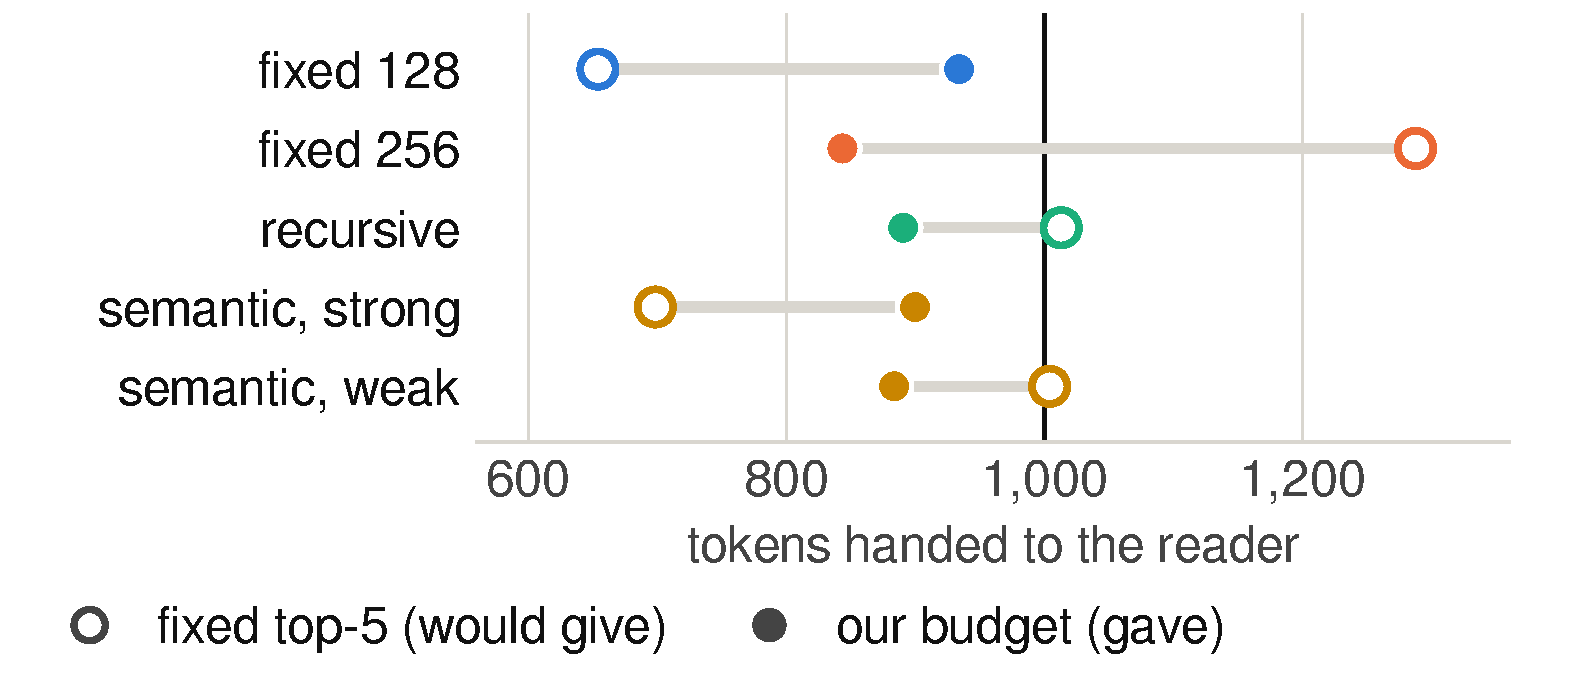
\includegraphics[width=\colw]{figures/fig_budget.pdf}

\lead{Reader and metrics.} Qwen2.5-3B-Instruct \citep{qwen2025qwen25},
4-bit \citep{dettmers2023qlora}, greedy, allowed to answer NO\_ANSWER.
Answer recall \citep{karpukhin2020dpr} and exact match, EM
\citep{rajpurkar2016squad}.

\lead{Statistics.} Paired bootstrap \citep{efron1993bootstrap}, exact
McNemar \citep{mcnemar1947}, Holm correction \citep{holm1979}, and a
minimum detectable effect (MDE) for every test \citep{card2020power}.

\lead{Code and data:}\\
\href{https://\repourl}{\bfseries\repourl}
\end{col}\hspace{\gut}%
\begin{col}
\sect{3}{Results}

\sub{RQ1: no moderation}
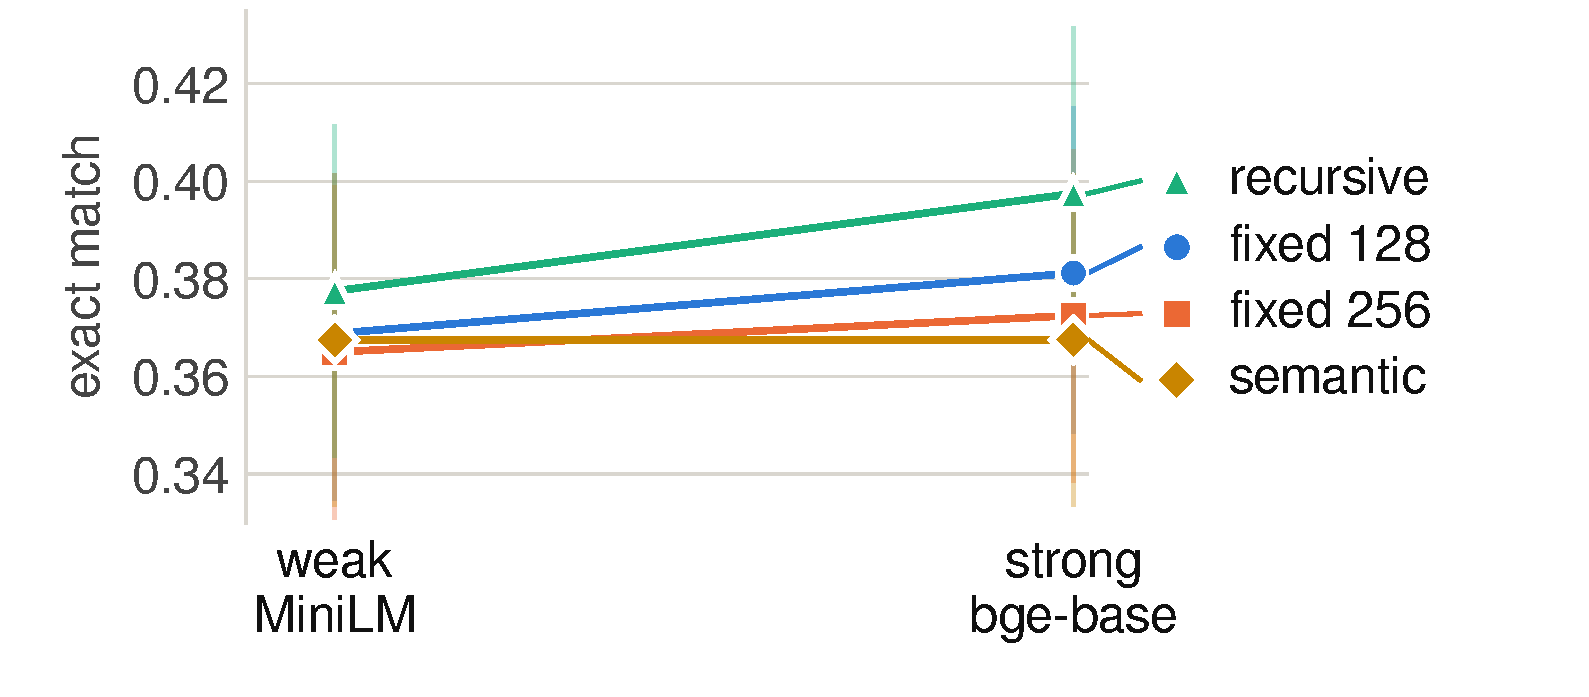
\includegraphics[width=\colw]{figures/fig_interaction.pdf}
\figcap{Exact match, 800 test questions; whiskers: 95\,\% CIs.}

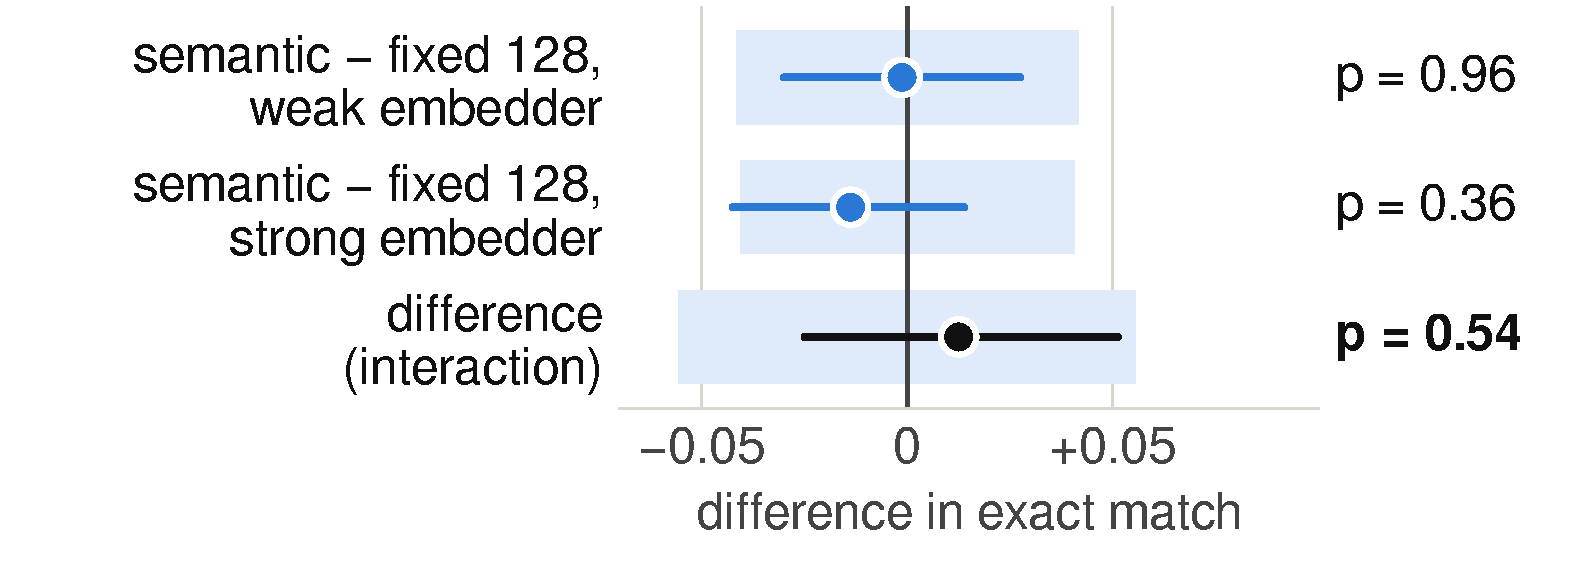
\includegraphics[width=\colw]{figures/fig_effects.pdf}
\figcap{Shaded: effects below each test's MDE (80\,\% power).}

\begin{verdict}
\lead{H1 not supported.} Interaction +0.013, 95\,\% CI
[\textminus 0.025, 0.051], \textit{p} = 0.54, MDE 0.056. Lenient EM and answer recall agree; none of 12
pairwise chunker contrasts survives Holm.
\end{verdict}
\end{col}

\vspace{3mm}
{\color{accent}\rule{\linewidth}{0.8mm}}
\vspace{1mm}

% ================================================= results, continued (RQ2)
\noindent
\begin{col}
\sub{RQ2: the reader is the bottleneck}
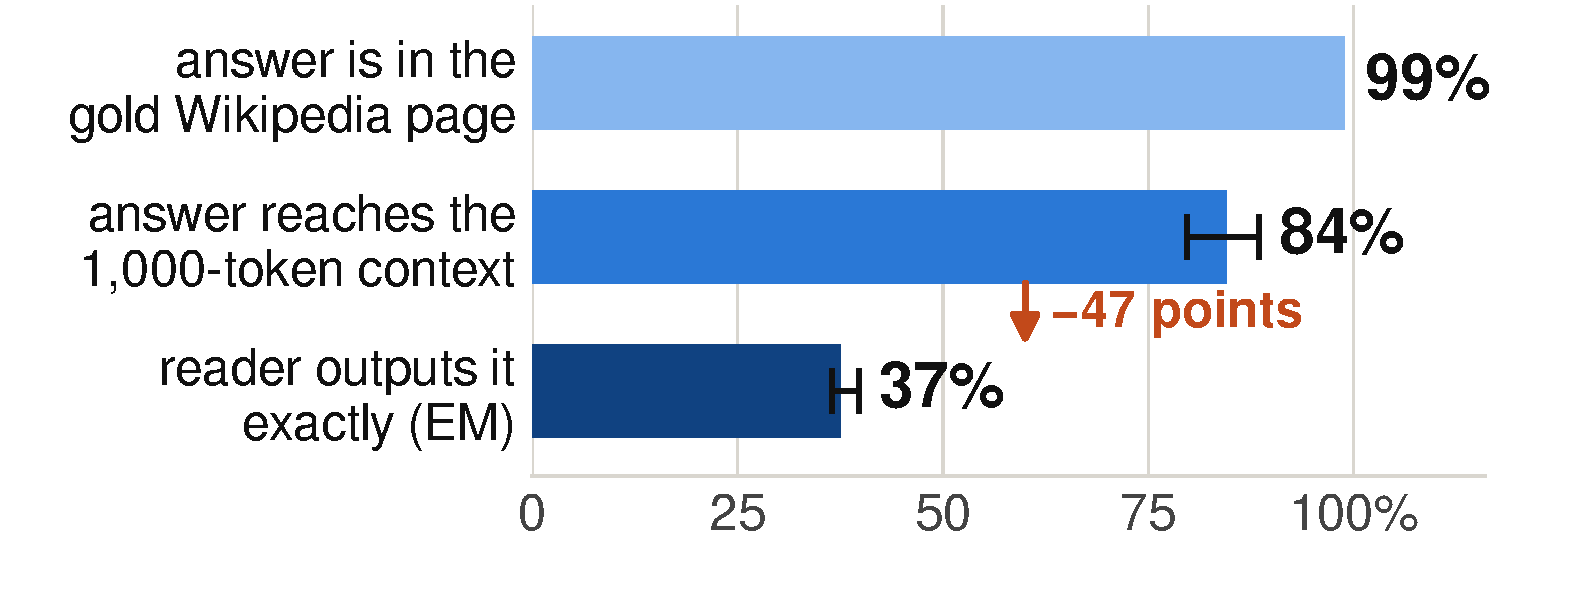
\includegraphics[width=\colw]{figures/fig_funnel.pdf}
\figcap{Mean of the 8 conditions; rules show their range.}

\lead{H2 not supported.} Even when the answer \emph{is} in the context, EM is
only 0.43--0.46 in every condition, and the reader declines 15--20\,\% of
those questions.
\end{col}\hspace{\gut}%
\begin{col}
\sub{Discussion}
\lead{Unexpected.} Chunking does move retrieval, and more for the weak
embedder (recall spread 0.038 vs 0.025), as H1 predicted. The reader absorbs
it: the EM spread is 0.013 (weak) vs 0.030 (strong).

\lead{Limitations.} One 3B reader, so the null may be reader-limited;
answers only at the 1,000-token budget; a gold-page corpus inflates
absolute recall; 200 dev questions for tuning.

\begin{tcolorbox}[colback=navy, colframe=navy, arc=3mm, boxrule=0pt,
                  left=7mm, right=7mm, top=4mm, bottom=4mm,
                  before upper=\RaggedRight]
\color{white}{\bfseries Take-away.}\hspace{0.35em}At a fixed context budget,
chunking choices barely reach the answer. Improve how the reader uses its
context before tuning the chunker.
\end{tcolorbox}
\end{col}

% every entry is cited invisibly so the poster numbers its references
% exactly as the appendix does (both use plainnat's alphabetical order)
\nocite{*}
\bibliographystyle{plainnat}
\nobibliography{refs}
\end{document}
